\input{../header}
\hyphenpenalty=5000

\rhead{Your name: \rule{8cm}{0.15mm}}

\begin{document}

\section{Learning target I2, version 1}

Given appropriate data about a function, determine outputs, direction, and concavity of its antiderivative, and/or construct an accurate graph.

\hrulefill

Consider the piecewise linear function $y = g(x)$ pictured below; assume that $g(x) = 0$ for $x \le -9$ and $x \ge 0$.
	
	\begin{center}
		\scalebox{0.33}{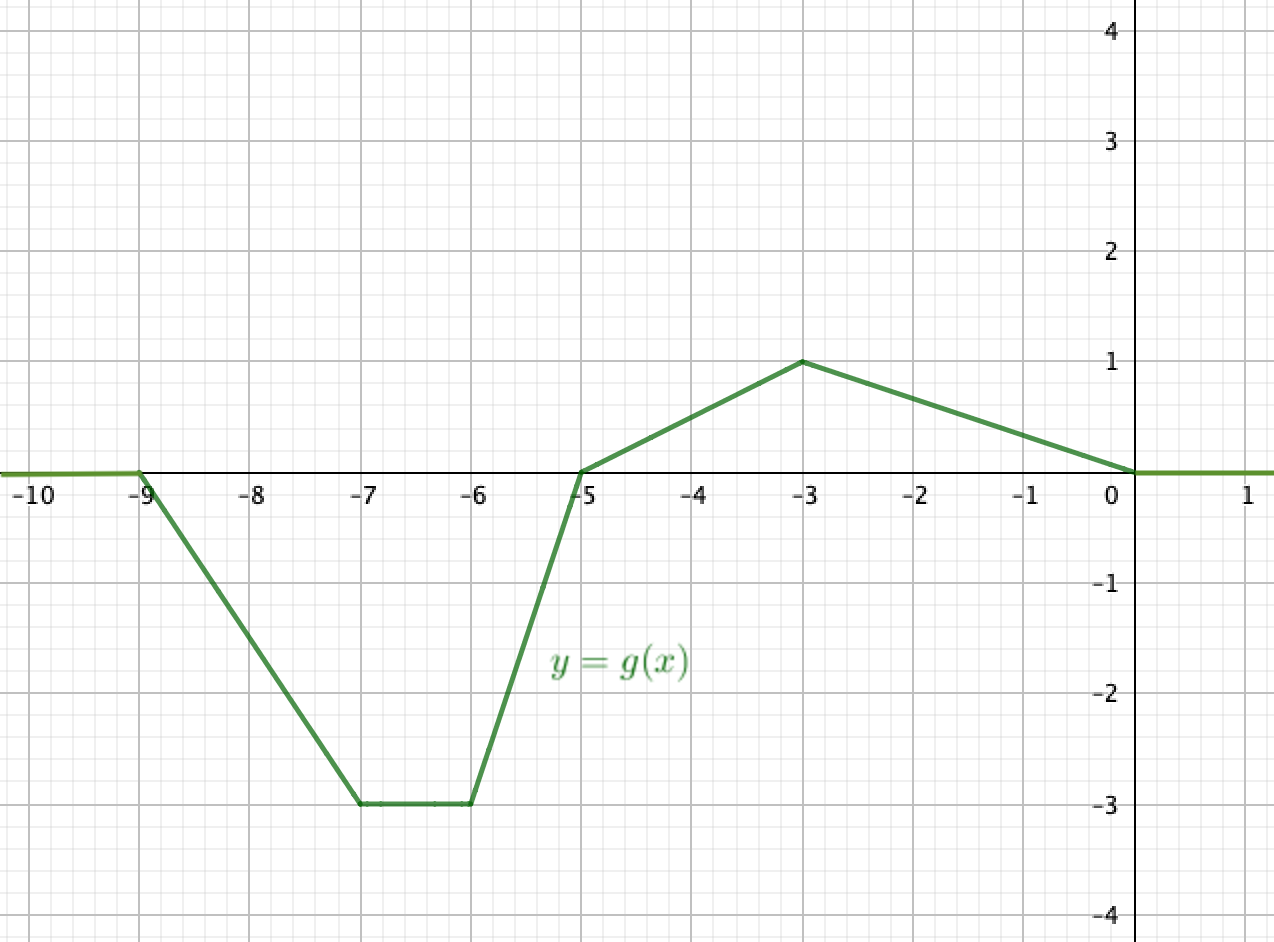
\includegraphics{images/CP11-LT14-11.png}} \hspace{0.5in} \scalebox{0.36}{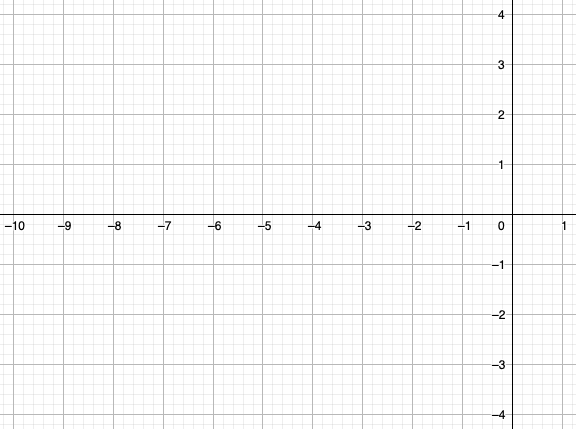
\includegraphics{images/CP-2-LT2-grid.png}} 
	\end{center}
	
	Let $G$ be an antiderivative of $g$ that satisfies $G(-9) = 3$.
	
	\begin{enumerate}[leftmargin=0pt]
		\item On what intervals is $G$ increasing?  decreasing? neither?  Carefully explain your answers.
		
		\vfill
		
		\item On what intervals is $G$ concave up?  concave down?  neither?  Carefully explain your answers.
		
		\vfill
		
		\item Recall we are given that $G(-9) = 3$.  Find the exact values of $G(-7)$, $G(-6)$, $G(-5)$, $G(-3)$, and $G(0)$.  Write one sentence to explain briefly how you found these values.
		
		\vfill
    \vfill
		
		\item On the blank grid at right, sketch an accurate, labeled graph of $y = G(x)$.
		
  \end{enumerate}

%%%%%%%%%%%%%%%%%%%%%%%%%%%%%%%%%%%%%%%%%%%%%%%%%%%%%%%
\pagebreak

\section{Learning target I2, version 2}

Given appropriate data about a function, determine outputs, direction, and concavity of its \\
antiderivative, and/or construct an accurate graph.

\hrulefill

Consider the piecewise linear function $y = f(x)$ pictured below; assume that $f(x) = 0$ for $x \le 0$ and $f(x) = 1$ for $x \ge 11$.
	
	\begin{center}
		\scalebox{0.33}{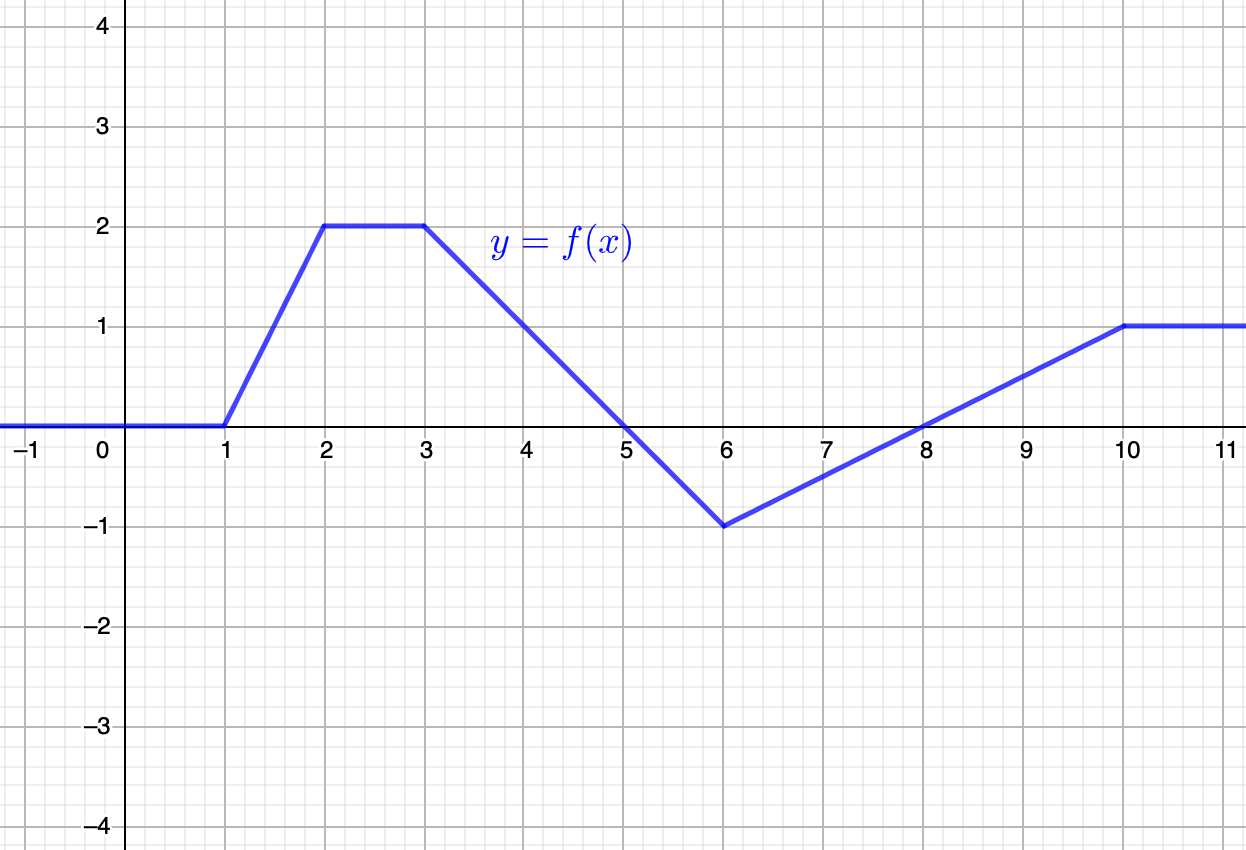
\includegraphics{images/CP-3-LT2-graph.png}} \hspace{0.2in} \scalebox{0.36}{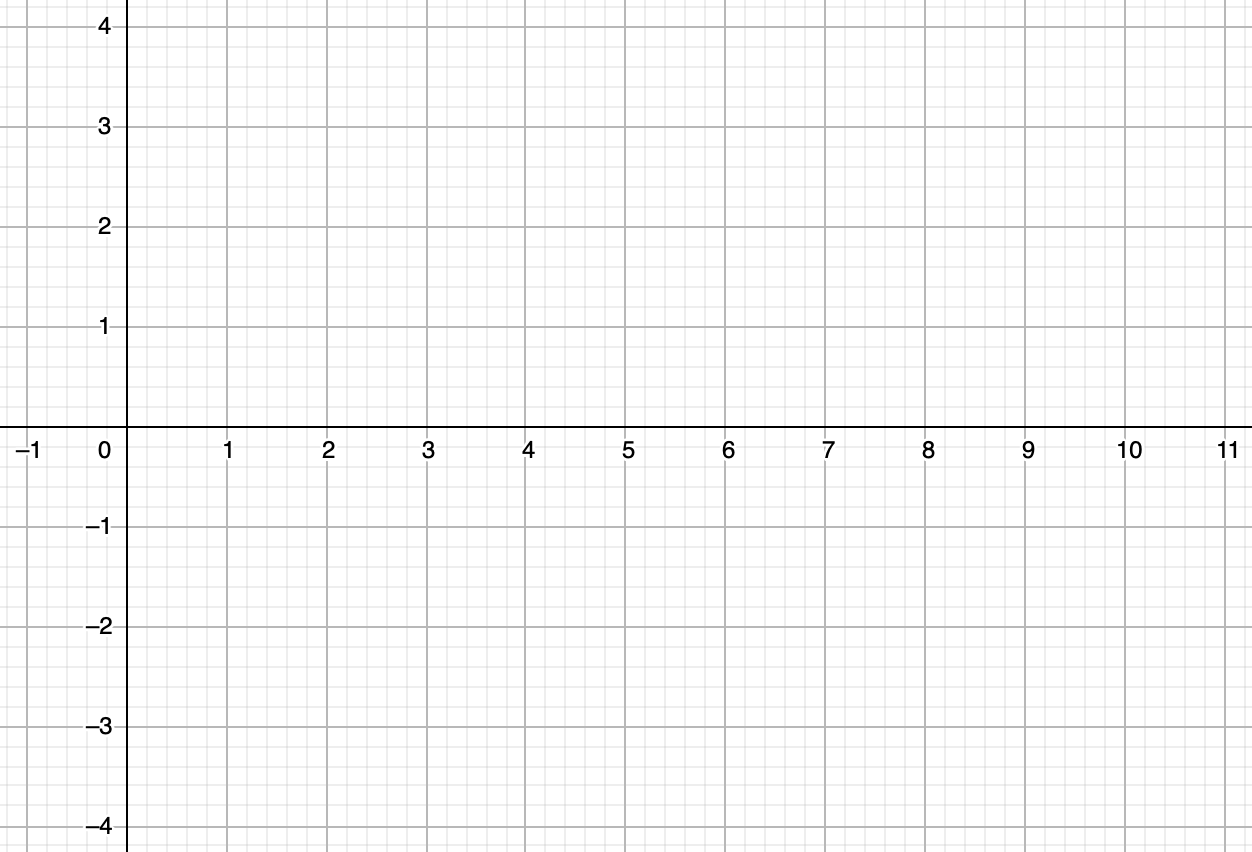
\includegraphics{images/CP-3-LT2-grid.png}} 
	\end{center}
	
	Let $F$ be an antiderivative of $f$ that satisfies $F(1) = -2$.
	
	\begin{enumerate}[leftmargin=0pt]
		\item On what intervals is $F$ increasing?  decreasing? neither?  Carefully explain your answers.
		
		\vfill
		
		\item On what intervals is $F$ concave up?  concave down?  neither?  Carefully explain your answers.
		
		\vfill
		
		\item Find the exact values of $F(2)$, $F(3)$, $F(5)$, $F(6)$, $F(8)$, and $F(10)$.  Write one sentence to explain briefly how you found these values.
		
		\vfill
    \vfill
		
		\item On the blank grid at right, sketch an accurate, labeled graph of $y = F(x)$.
		
  \end{enumerate}

\pagebreak
%%%%%%%%%%%%%%%%%%%%%%%%%%%%%%%%%%%%%%%%%%%%%%%%%%%%%%%

\section{Learning target I2, version 3}

Given appropriate data about a function, determine outputs, direction, and concavity of its \\
antiderivative, and/or construct an accurate graph.

\hrulefill


Consider the piecewise linear function $y = f(x)$ pictured below; assume that $f(x) = 0$ for $x \le -1$ and $f(x) = 1$ for $x \ge 11$.
	
	\begin{center}
		\scalebox{0.35}{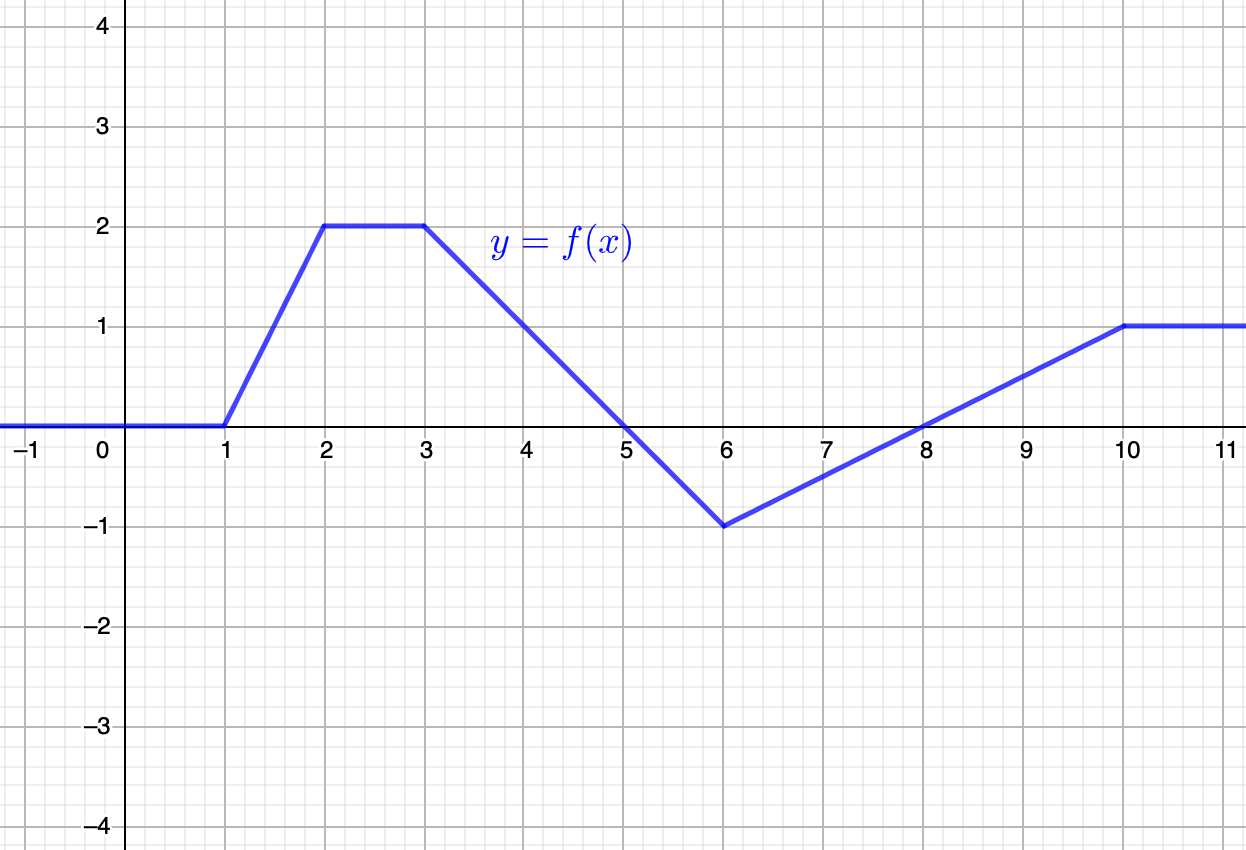
\includegraphics{images/CP-3-LT2-graph.png}} \hspace{0.25in} \scalebox{0.35}{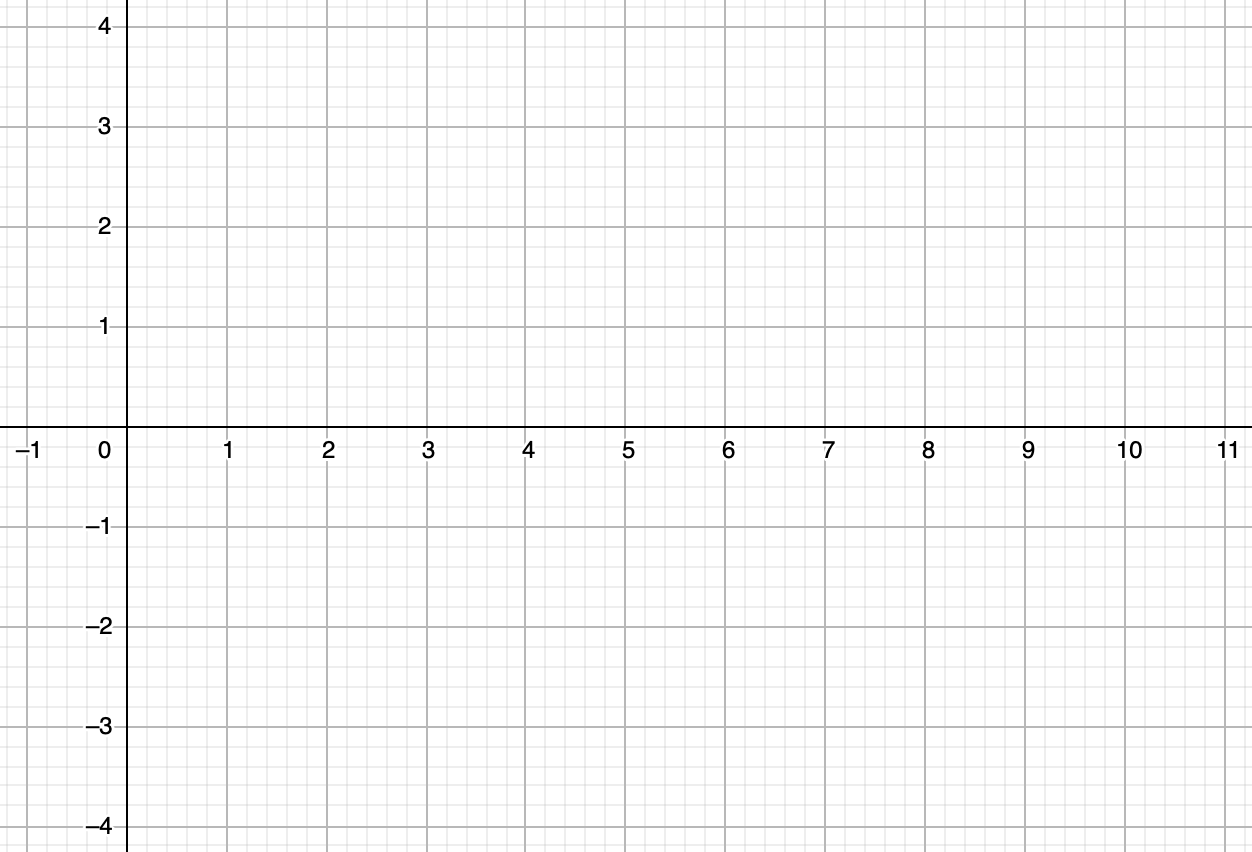
\includegraphics{images/CP-3-LT2-grid.png}} 
	\end{center}
	
	Let $F$ be an antiderivative of $f$ that satisfies $F(1) = -2$.
	
	\begin{enumerate}[leftmargin=0pt]
		\item On what intervals is $F$ increasing?  decreasing? neither?  why?
		
		\vfill
		
		\item On what intervals is $F$ concave up?  concave down?  neither?  why?
		
		\vfill
		
		\item Find the exact values of $F(2)$, $F(3)$, $F(5)$, $F(6)$, $F(8)$, and $F(10)$.  Write one sentence to explain briefly how you found these values.
		
		\vfill
		\vfill
		
		\item On the blank grid at right, sketch an accurate, labeled graph of $y = F(x)$.
		
	\end{enumerate}

\end{document}